\chapter{Open Air Museum versione 2.0}
\vspace{5mm}

\section{Server}\vspace{5mm}

L'applicativo lato server è stato riscritto interamente ma le sue funzionalità  sono rimaste invariate. Le modifiche apportate infatti riguardano principalmente le tecnologie. Ora la gestione del database viene fatta attraverso un ORM chiamato Sequelize che offre una serie di funzionalità fondamentali: in primis dà la possibilità, nel caso dell'utilizzo di SqLite come tecnologia, di generare un database all'avvio dell'applicativo se al percorso indicato non esiste alcun file di SqLite. Inoltre genera la struttura del database utilizzando la dichiarazione di modelli che avvengono mediante le sue API. Infine offre la possibilità di astrarre le query tramite un'interfaccia più familiare a Javascript senza obbligare il programmatore a generarle tramite concatenazione di stringhe o altri metodi. Il framework utilizzato per il routing delle api è Express.\vspace{5mm}

Quello che differenzia la vecchia implementazione rispetto alla nuova, è una serie di endpoint che permette di gestire e inviare la configurazione degli applicativi lato client in modo da centralizzare il più possibile la personalizzazione degli applicativi mobile e dell'applicativo admin.  

\section{Applicativo Admin}\vspace{5mm}

Il compito dell'applicativo admin è quello di sostituire quello in Filemaker ed espandere alcune delle sue funzionalità. Come descritto in precedenza, questo applicativo è stato sviluppato come una SPA utilizzando React come framework di sviluppo. Le feature che possiede sono: la possibilità di modificare testi e media per i vari punti e percorsi di interesse, la possibilità di creare percorsi selezionando e ordinando punti precedentemente creati e la capacità di poter monitorare l'utilizzo della piattaforma attraverso un pannello che mostra i punti più visitati e i percorsi più seguiti. L'accesso a tale applicativo è possibile solo attraverso autenticazione contro il server mediante le Rest Api da esso fornite.\vspace{5mm}

\section{Modello ER}\vspace{5mm}

Ora descriverò brevemente il nuovo schema logico dell'applicativo e come le varie tecnologie, tutte basate su Javascript, interagiscono fra loro.

\vspace{5mm}Come si può vedere in figura 3.2 lo stack tecnologico risulta meno complesso e vanta l'utilizzo di un numero minore di tecnologie per raggiungere le medesime funzionalità. Come si può notare i punti di interazione con la piattaforma sono gestiti da due applicativi basati entrambi su React: il primo è l'applicativo mobile che utilizza React-Native mentre il secondo è la webApp admin. Entrambi ricevono input dall'utente, ma il primo utilizza hardware esterno per arricchire la propria raccolta informazioni. Infatti la posizione dell'utente è individuata attraverso il Gps o il Bluetooth. Tali applicativi interagiscono con il server mediante delle Rest Api che, come nella versione precedente, forniscono i dati sui punti e i percorsi. A differenza del primo l'applicativo, però, portano anche la configurazione impostata dal lato admin, in modo da adattarlo alle richieste di chi gestisce i punti e i percorsi. Tali dati vengono salvati in un database SqLite il cui unico punto di accesso è attraverso le API fornite dal server. Lo schema ER di questa nuova versione è quello mostrato in figura 3.1.

\begin{figure}[h]
\centering
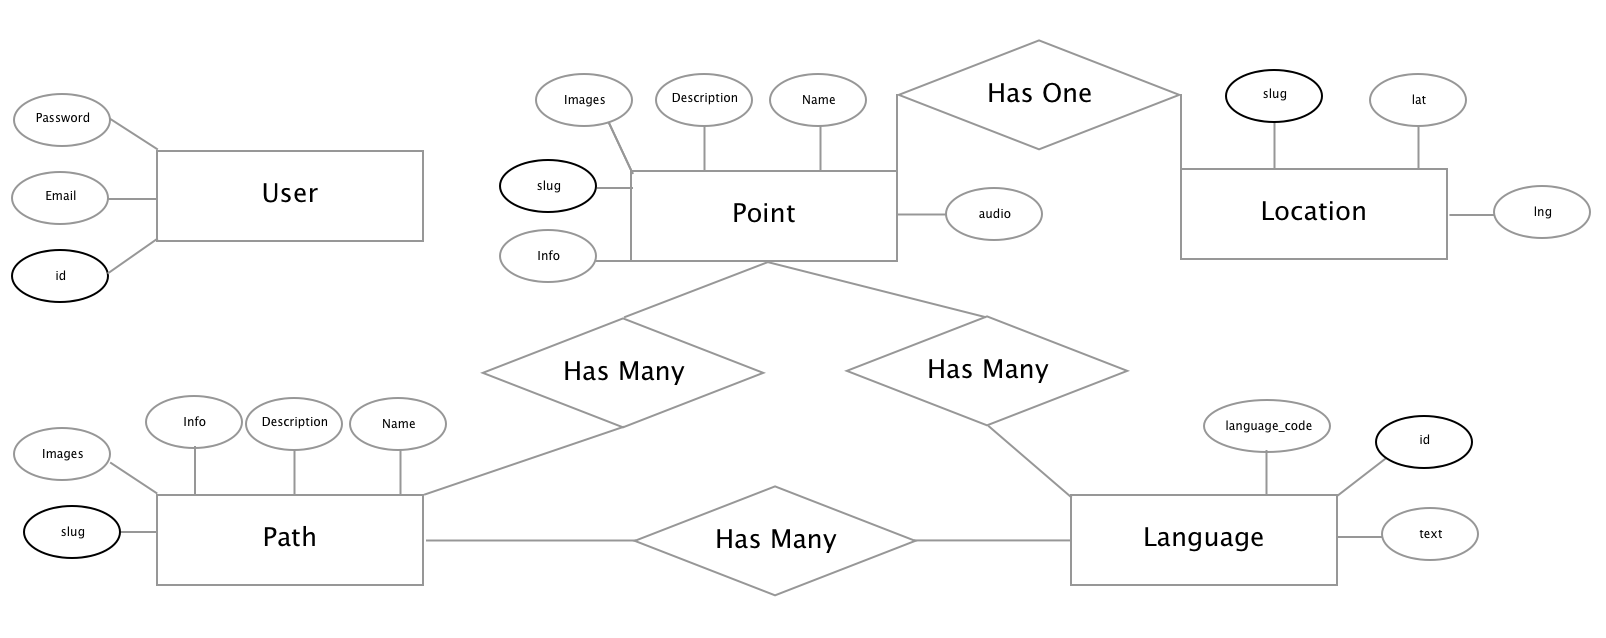
\includegraphics[width=0.9\textwidth]{images/erNew.png}
\caption{Schema ER nuova versione}
\end{figure}

Utilizzare il server come fonte di verità per tutti gli applicativi garantisce che i dati siano sempre consistenti con quello che è l'applicativo server, in modo da mantenere la struttura consistente con il versionamento del prodotto. Un ulteriore struttura per mantenere i dati è presente a lato mobile mediante Redux. Questo è utile per poter salvare le configurazioni e mantenerle tali in modo consistente attraverso l'app al fine di creare una coesione tra tutti i componenti di React che necessitano di usufruire dei dati. Tale stato applicativo viene idratato attraverso le api Rest, e quando questo non è possibile per mancanza di rete, permette di utilizzare tramite React-native lo Storage locale del dispositivo come luogo di backup. Ogni mutazione dello stato applicativo viene infatti seguita da un'operazione asincrona che ha lo scopo di salvare uno snapshot dello store nella memoria del dispositivo. In questo modo è garantita consistenza nel mostrare gli ultimi dati disponibili anche se il dispositivo risulta offline.\vspace{5mm}

\begin{figure}[h]
\centering
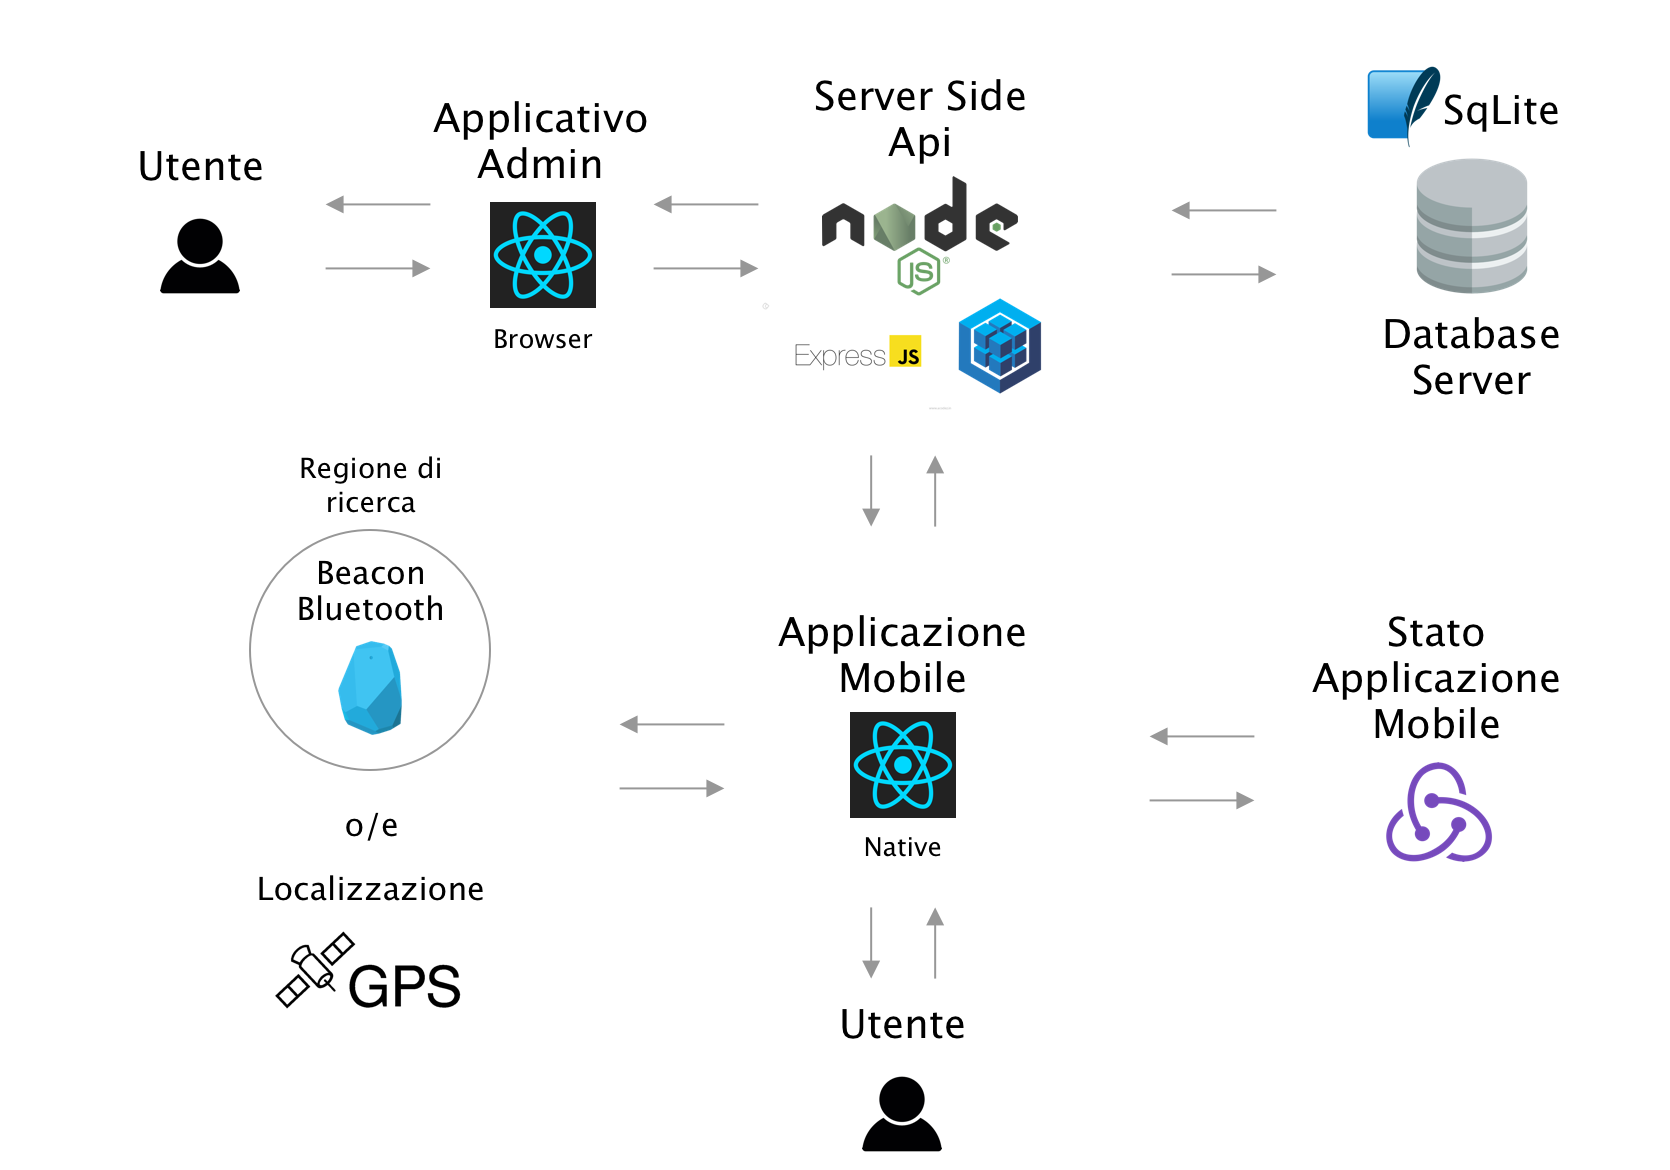
\includegraphics[width=0.8\textwidth]{images/stackAlakai.png}
\caption{Schema logico della struttura 2.0}
\end{figure}


\section{Porting applicativi Nativi}\vspace{5mm}
\emph{Ora verrà descritto nel dettaglio il porting degli applicativi nativi a React-native, il percorso implementativo e i punti critici.}
\vspace{5mm}
\subsection{Caratteristiche principali}\vspace{5mm}

La caratterizzazione fondamentale di questo tipo di porting è quello di non compromettere la funzionalità iniziale dell’applicativo, mantenendo un \emph{look-and-feel} il più possibile vicino a quello iniziale e apportando le possibili migliorie date dal nuovo ambiente. La prima problematica affrontata è stata quella di poter gestire la modalità Esplora da Javascript: ovvero essere in grado di controllare il bluetooth dello smartphone e monitorare l’avvicinarsi a specifiche aree marcate dai Beacon, mediante l'utilizzo di task in background. La versione nativa si avvale della tecnologia iBeacon sfruttata dall'SDK di Estimote. E' stato deciso di mantenerla anche nella seconda versione, vista la presenza di hardware già configurato sul territorio.  \vspace{5mm}

Come detto in precedenza, la comunicazione tra il reame nativo e quello Javascript avviene attraverso una particolare struttura software chiamata bridge. Tramite le Api messe a disposizione da React-Native è possibile utilizzare questa struttura per trasferire i dati. \vspace{5mm}

I paragrafi seguenti descrivono nel dettaglio in che modo utilizzare tali api per garantire nel reame Javascript le stesse Api dell’SDK Estimote proximity, sia su iOS che su Android.\vspace{5mm}

Per quanto riguarda iOS, è necessario aggiungere alle dipendenze del progetto, l'Estimote Proximity SDK utilizzando CocoaPods, un dependency manager per XCode. Inoltre, per abilitare la localizzazione in background, è necessario aggiungere tra le \emph{capabilities} dell’applicativo nella sezione \emph{Background Mode} la voce \emph{Uses Bluetooth LE accessories}. \vspace{5mm}

Il passo successivo consiste nel creare un file che permetta di dichiarare ed esportare i metodi di configurazione e gestione della libreria di Estimote. Per fare questo si utilizza l’interfaccia fornita da RCTBridgeModule di React-Native, in modo da rendere visibili i metodi dichiarati nel codice nativo al lato Javascript quando l'applicativo viene compilato ed eseguito. Un ulteriore punto fondamentale riguarda la comunicazione attraverso il “bridge”: tale procedura è asincrona e per questo è possibile passare valori da nativo a Javascript solamente mediante callback o eventi. \vspace{5mm}

Nel caso specifico, la scelta è ricaduta su di un sistema ad eventi, vista la maggior flessibilità di utilizzo. In particolare i metodi messi a disposizione attraverso il “bridge” sono:\vspace{5mm}

\begin{itemize}
	\item initialize:(NSDictionary *)config
	\item startObservingZones:(NSArray *)zonesJSON
	\item stopObservingZones()
\end{itemize}\vspace{5mm}
	
Il primo ha lo scopo di inizializzare l'SDK Estimote attraverso un oggetto che contiene i vari parametri di configurazione. Il secondo permette di mettere il device in ascolto su una lista di regioni identificate mediante dei tag. Nel momento in cui un telefono entrerà in una zona così configurata verrà lanciato l’evento “Enter” dal reame nativo a Javascript attraverso il bridge. Per l’uscita da una regione verrà lanciato l’evento “Exit” mentre per un cambio di contesto mentre si è in una zona verrà lanciato l'evento “Change”. Il contesto è un parametro passato nella funzione chiamata dalla sottoscrizione a questi eventi e contiene le informazioni del Beacon che rappresenta quella regione.\vspace{5mm}

Per quanto riguarda Android lato Javascript, le api sono le medesime. Questo per dare una sensazione di uniformità tra le due piattaforme. Per quanto riguarda l’implementazione nativa: l'uso dell’SDK avviene nello stesso modo di iOS; così come l’esportazione dei metodi attraverso il “bridge”. Ciò che cambia effettivamente sono solo le configurazioni necessarie date dal diverso tipo di ambiente (Java).\vspace{5mm}

A questo punto mediante un interfaccia messa a disposizione da React-Native è possibile quindi utilizzare i metodi esportati dalle due piattaforme. Tali metodi sono esportati attraverso l’oggetto \emph{NativeModules} che a sua volta contiene un oggetto per ogni classe che implementa l’interfaccia RCTBridgeModule. In seguito è stato scelto di utilizzare un file Javascript che normalizzasse l’esportazione dei vari metodi.\vspace{5mm}

Il risultato ottenuto da questa implementazione ha permesso di ottenere delle api paritetiche lato Javascript, nonostante le grandi differenze tra i due sistemi operativi. Questo offre un astrazione che elimina la complessità di dover gestire singolarmente due linguaggi diversi con ambienti diversi. \vspace{5mm}

Quindi mediante le “Bridge Api”, React-Native offre la possibilità di costruire librerie non \emph{cross-platform} ma \emph{multi-platform}. Tale valore non è indifferente e può risultare cruciale per quanto riguarda tempi di sviluppo e feature del prodotto, dando la possibilità di scrivere solo il codice nativo necessario e sviluppando poi il resto della logica in un'ottica \emph{“write once run anywhere”}.\vspace{5mm}

Dal punto di vista grafico, inoltre, sono state apportate molte modifiche date dai feedback di molti utenti che trovavano l’applicativo precedente poco intuitivo. Si è passati da una visualizzazione dei punti di interesse da lista a mappa. Infatti molti utenti si lamentavano del fatto che non era immediato capire dove fossero i punti rispetto alla loro posizione.\vspace{5mm}

\begin{figure}[h]
\centering
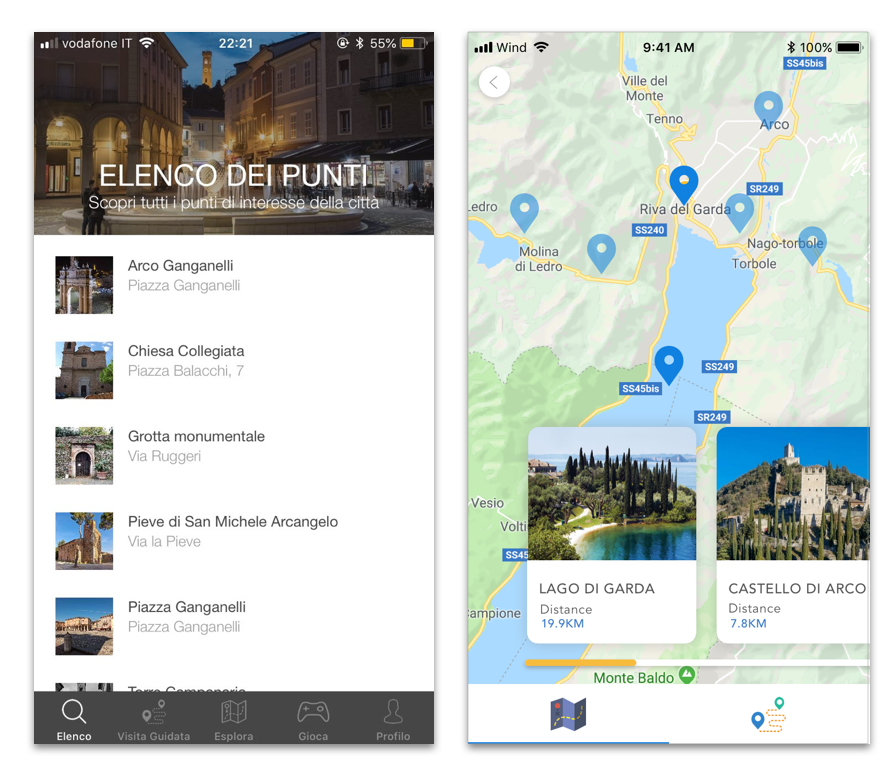
\includegraphics[width=0.7\textwidth]{images/punti.png}
\caption{Confronto HomeScreen Open Air Museum vecchia e nuova versione}
\end{figure}

\begin{figure}[h]
\centering
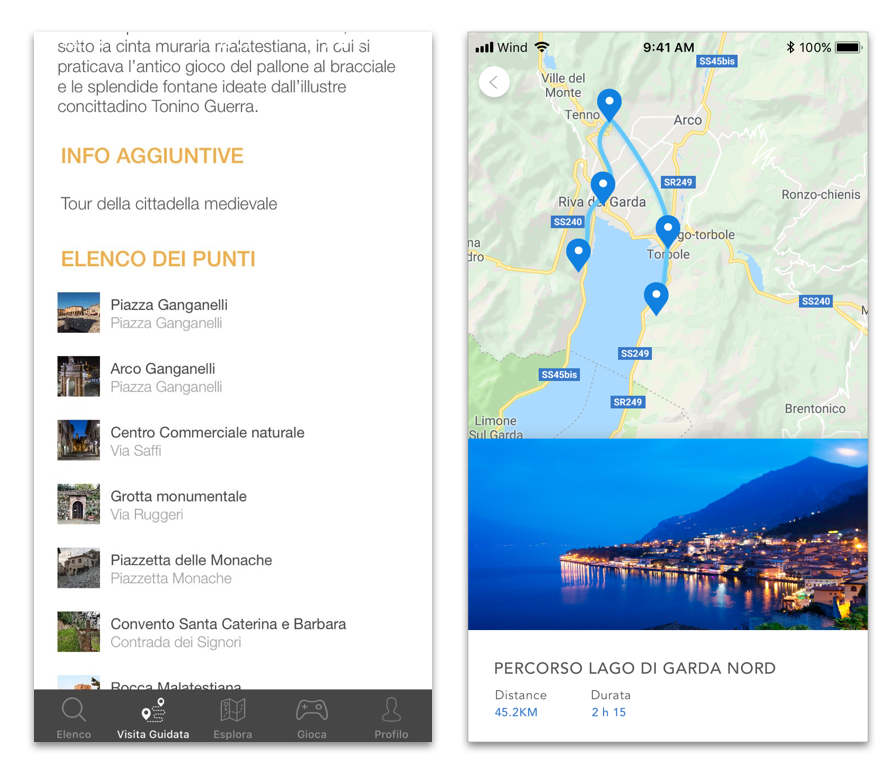
\includegraphics[width=0.6\textwidth]{images/percorsi.png}
\caption{Confronto HomeScreen Open Air Museum vecchia e nuova versione}
\end{figure}\vspace{19mm}

Sfruttando la potente libreria di animazioni fornita da React-Native è stato possibile creare un'interfaccia ricca e moderna mantenendo le prestazioni elevate anche su dispositivi non recenti e di alta fascia. Il “driver” di tale libreria è infatti nativo ed implementato nel modo più efficiente per i due sistemi operativi. Questo offre solide prestazioni anche nel caso di animazioni molto complesse ma aggiunge anche alcune limitazioni. La più evidente è l’obbligo di implementare tali animazioni con un pattern dichiarativo: indicando quindi in precedenza il modo in cui l’oggetto deve comportarsi per poi avere la possibilità di eseguirlo mediante un'interfaccia di start e stop.

\begin{figure}[h]
\centering
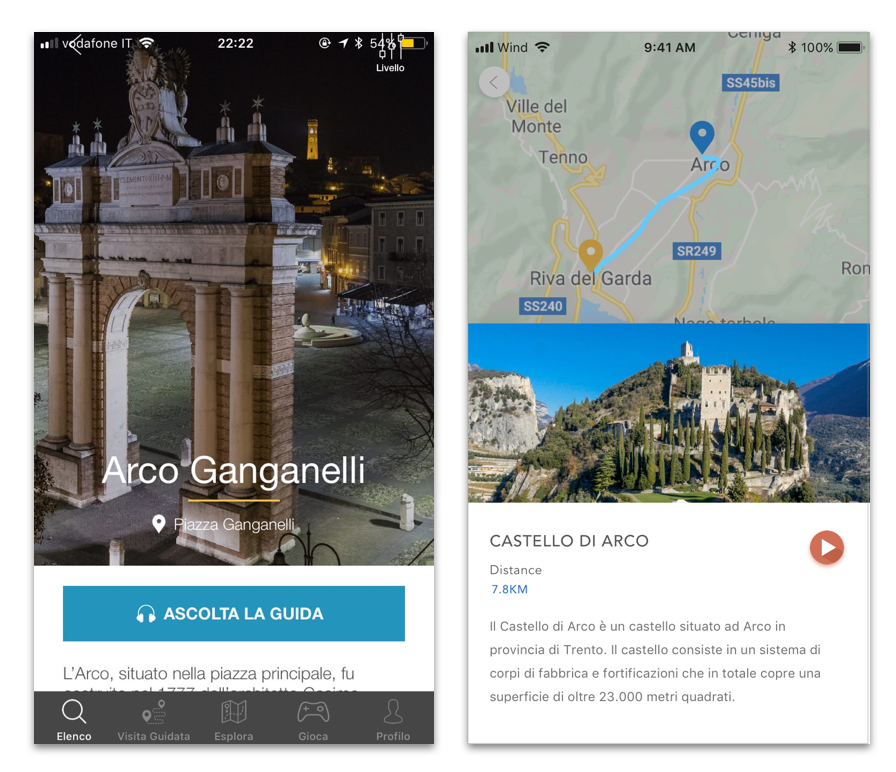
\includegraphics[width=0.6\textwidth]{images/audio.png}
\caption{Confronto HomeScreen Open Air Museum vecchia e nuova versione}
\end{figure}

Un'ulteriore funzionalità richiesta dal porting è stata quella di poter riprodurre dei contenuti audio all’interno dell’applicativo. In particolare questi contenuti sono presenti sul server e sono serviti attraverso un'api che permette il loro streaming. In precedenza era stato sviluppato un player che utilizzava i rispettivi SDK nativi per controllare l’audio. L'utente era in grado di avviare e stoppare l’audio e proseguire avanti veloce mediante una barra di trascinamento. Le funzionalità per i due sistemi operativi erano le stesse ma vista le diversità tra le due piattaforme è stato necessario re-implementare la stessa logica due volte.\vspace{2mm}

Utilizzando React-native è stato possibile scrivere la logica una sola volta e condividerla tra le due piattaforme utilizzando un package open source chiamato \emph{react-native-audio-streamer}. Il package permette di configurare uno stream audio mediante una url e di controllarne la riproduzione. Le API lato javascript sono le medesime seppur a lato nativo il package utilizzi due librerie diverse: per Ios \emph{DuoAudioStreamer} e per Android \emph{ExoPlayer}. L’utilizzo di tale package ha accelerato lo sviluppo, mostrando il vantaggio di React-native sopra a soluzioni simili: la maturità dell'ecosistema. Creare una dipendenza esterna in un progetto enterprise come questo può essere una scelta rischiosa. Legarsi ad un software di terze parti per una feature cruciale dell’applicativo può sfociare in problematiche che spaziano dal mantenimento futuro a bug non facilmente tracciabili. Ma, data la semplicità di questa particolare libreria, tale rischio è ragionevolmente contenuto.\vspace{2mm}

Come si è visto, l’impiego di React-native non ha soppiantato la totalità della parte nativa, anzi questo approccio “misto” ha permesso di non trovarsi limitati da una tecnologia rispetto ad un altra, offrendo sempre il giusto tool per la feature richiesta. Durante le ricerche legate allo sviluppo di questo prodotto non sono stati trovati linguaggi o framework più flessibili e adatti alle molteplici configurazioni di questo progetto. Questo specifico caso è un ottimo esempio di come l’impiego di Javascript al di fuori dal browser sia la scelta vincente per creare un applicativo moderno e flessibile senza sacrificare manutenibilità e consistenza nel tempo.

\subsection{Implementazione di Redux}\vspace{5mm}

\begin{figure}[h]
\centering
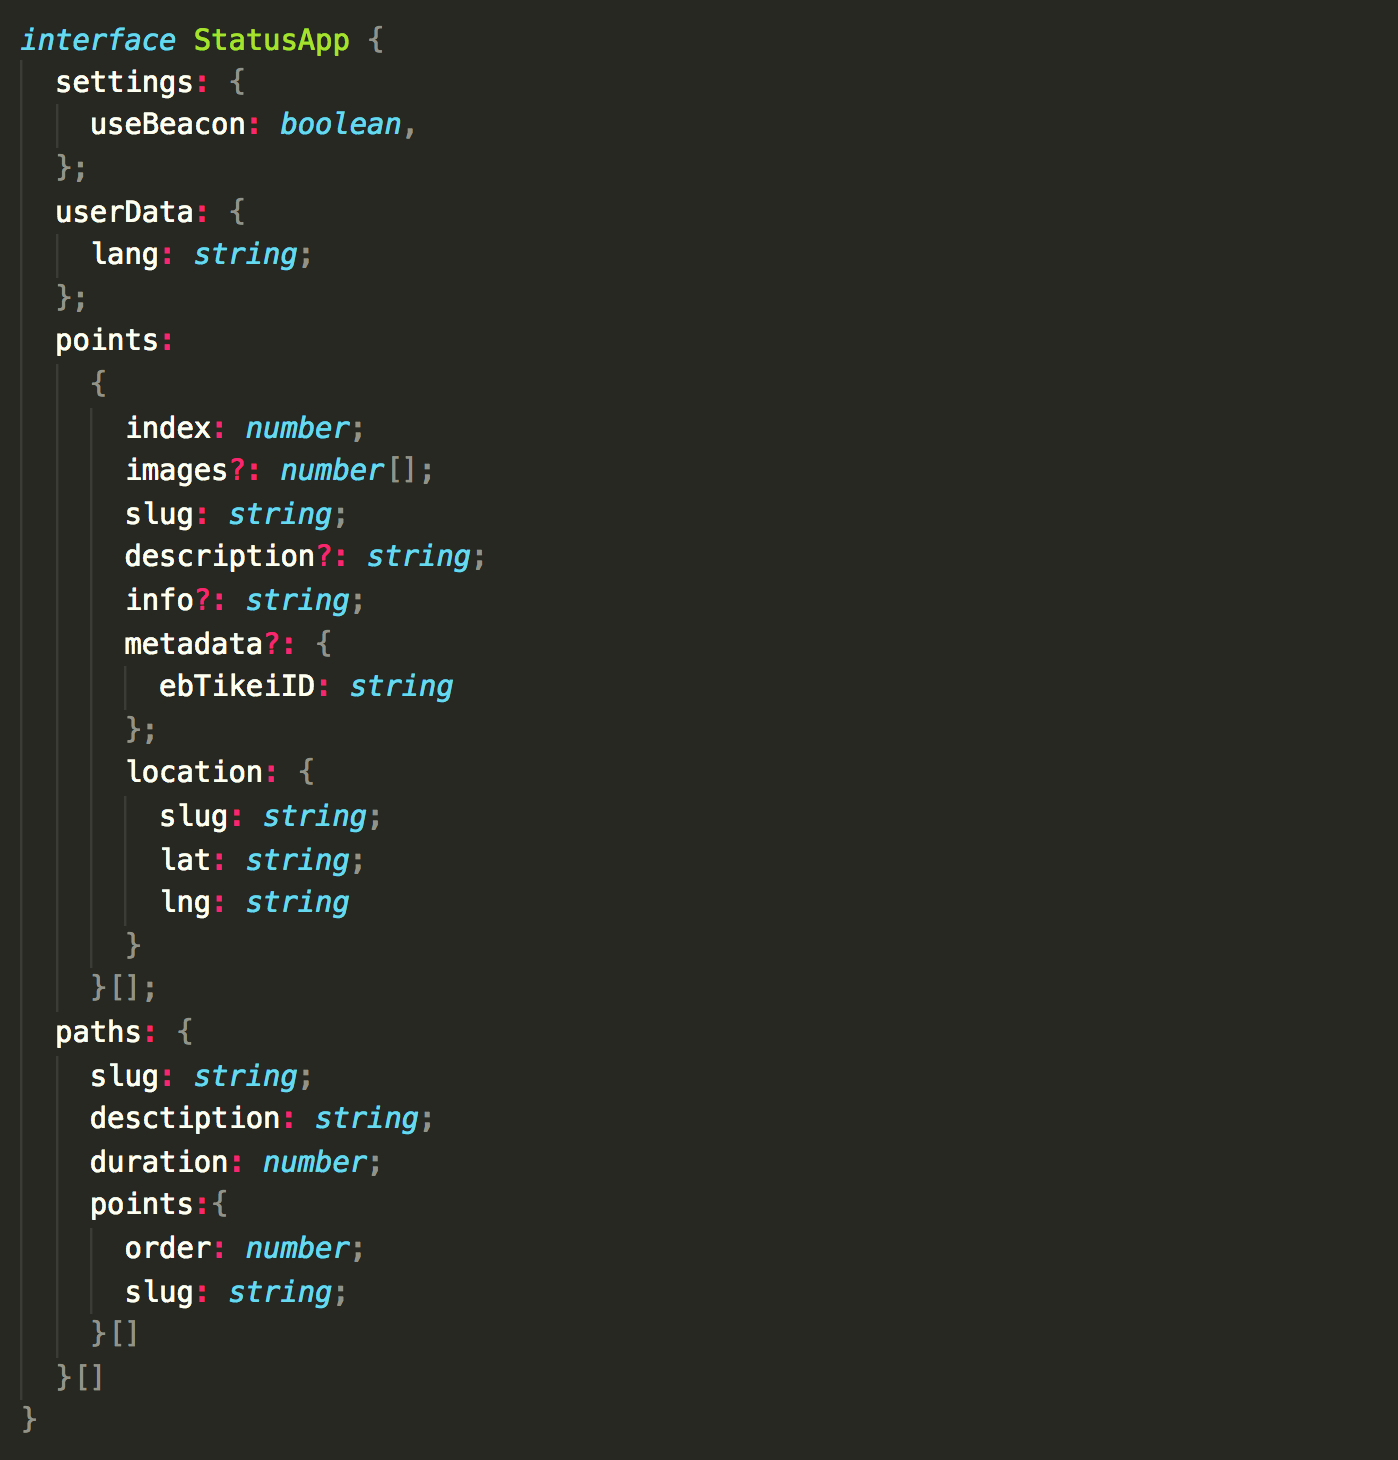
\includegraphics[width=0.7\textwidth]{images/store.png}
\caption{Interfaccia Store Redux}
\end{figure}

Per l'implementazione di Redux si è scelto di sviluppare una piccola libreria da condividere tra l'applicativo mobile e la web-app admin. Questa libreria comprende l'insieme dei Reducer e delle Action, disponibili sia nell'applicativo mobile che in quello web, e un costrutto software per usufruire delle Rest Api lato server. Questo approccio ha permesso di velocizzare notevolmente lo sviluppo, permettendo di riutilizzare la parte che gestiva il flusso logico applicativo e concentrandosi solamente sui componenti dediti alla visualizzazione grafica dei dati.\vspace{5mm}

Come si può vedere dalla figura 3.6, lo stato applicativo consiste in un oggetto immutabile che detiene tutti i dati necessari. Quindi oltre ai vari punti e percorsi, nello store, sono contenute anche le impostazioni relative all'applicativo specifico: come la lingua selezionata dall'utente o l'utilizzo o meno di iBeacon come sistema di localizzazione.\vspace{5mm}

\subsection{Mappa interattiva}\vspace{5mm}

Come si pùò vedere dalle figure 3.3, 3.4 e 3.5, il componente principale dell'interfaccia applicativa è composto da una mappa interattiva. Questo componente è messo a disposizione da una libreria chiamata \emph{react-native-maps} che offre una serie di feature come la generazione di \emph{marker} customizzati e la gestione delle interazioni con la mappa stessa attraverso eventi di \emph{pan} e \emph{drag}. E' stato scelto di utilizzare questo package, rispetto a quello sviluppato per la precedente versione, per via delle numerose funzionalità che la nuova interfaccia grafica richiede. Infatti l'implementazione proprietaria precedente è basata su Open Street Maps e non è in grado di supportare la generazione di percorsi. Mentre React-native-maps offre nativamente un canvas con cui è possibile disegnare sulla mappa tutti i poligoni necessari per la creazione di un percorso interattivo. \vspace{5mm}

\subsection{Punti critici e problematiche}\vspace{5mm}

Durante questo porting sono stati evidenziati una serie di punti critici implementativi: nei seguenti paragrafi sarà descritta la soluzione adottata per ogni problema specifico ed un'eventuale soluzione alternativa.\vspace{5mm}

L’utilizzo di una libreria esterna, come quella per la gestione degli stream audio o quella per la mappa, creano delle dipendenze che aggiungono una serie di incognite sulla longevità del prodotto. E’ importante legare il progetto il meno possibile a risorse esterne non del tutto affidabili. Per tale ragione entrambe le risorse esterne che l’applicativo utilizza e cioè la libreria per lo streaming audio e l’SDK Estimote sono gestite attraverso un layer software.\vspace{5mm}

 L’applicativo utilizza la libreria attraverso le Api fornite da questa interfaccia: in caso di necessità, si può sostituire più agevolmente la vecchia libreria con la nuova, mappando le nuove api sull’interfaccia. Ovviamente questo è possibile nei limiti di una coesione logica tra la il vecchio e nuovo SDK. Da notare che un'implementazione di questo tipo permette inoltre di abbandonare del tutto il software esterno, implementando la propria libreria e integrandola nel progetto facilmente attraverso tale interfaccia. Un ulteriore possibile soluzione a questo problema sarebbe quello di gestire internamente la maggior parte del software ma in alcuni casi questa soluzione deve essere scartata per l’elevato costo.\vspace{5mm}

Un'altra problematica è data dalla coesistenza di tre linguaggi differenti nella stessa codebase. In alcuni casi React-native può aggiungere complessità invece che rimuoverla: se la quantità di codice nativo a cui dover attingere è molto grande si rischia di dover mantenere tre ecosistemi a differenza di due. Maggiori sono le tecnologie da conoscere per operare su un prodotto, maggiore è il bagaglio necessario per mantenerlo. Questo rende il software più complesso da gestire. In questo caso un'attenta analisi del progetto prima dello sviluppo può guidare verso una soluzione differente ed evitare il problema.\vspace{5mm}

 Nel caso specifico di Open Air Museum 2.0, la quantità di codice nativo necessaria non è stata molta ma tale problema potrà presentarsi in futuro con il proseguire del progetto.\vspace{5mm}

Un alto punto critico da tenere in considerazione quando si effettua questo genere di porting è la completa scomparsa di database Sql in favore di uno \emph{state manager} ad oggetti. Data l'impossibilità di gestire i dati in modo paritetico rispetto alla versione nativa, è stato necessario riadattare la logica applicativa a questa nuova tecnologia. L'assenza dei tempi di latenza per accedere ai dati ha migliorato molto la forma del codice, che risulta molto più conciso e pulito.\vspace{5mm}

 La modifica dei dati avviene attraverso mutazioni allo stato. Questo comporta, in caso di applicativi molto grandi, una crescente complessità se non si dividono in modo accorto le varie aree dello stato: è possibile dividere in modo netto un'area dall'altra usando nodi il più possibile vicini alla radice. Tale approccio, infatti, permette di ottenere una buona \emph{separation of concerns}\cite{SOC} delle varie aree logiche dell'applicativo, ponendo entrypoint diversi per l'accesso ai dati, a seconda della zona logica prestabilita. Ciò permette di risolvere il problema descritto sopra, offrendo un guadagno in termini di semplicità rispetto ad una soluzione basata su SqLite.

